
\subsection{Geomety example: single pin}
\begin{frame}[fragile]
    \frametitle{Geometry of single pin cell}

    \begin{columns}
        \column{0.6\textwidth}
        \inputminted[frame=single,fontfamily=tt,fontsize=\tiny]{python}{examples/ex2_geom.py}

        \column{0.4\textwidth}{\scriptsize
        \begin{itemize}
            \item Solid's dimensions can be specified using correspondent attributes    
            \item Solid can be inserted into another
            \item Solid can be positioned with respect to its container
            \item \pythoninline/colormap/ function uses Matplotlib
        \end{itemize}
        }
     \end{columns}
\end{frame}

\begin{frame}[fragile]
    \frametitle{Plots}
    \begin{columns}
        \column{0.5\textwidth}
            {\tiny z plane}
            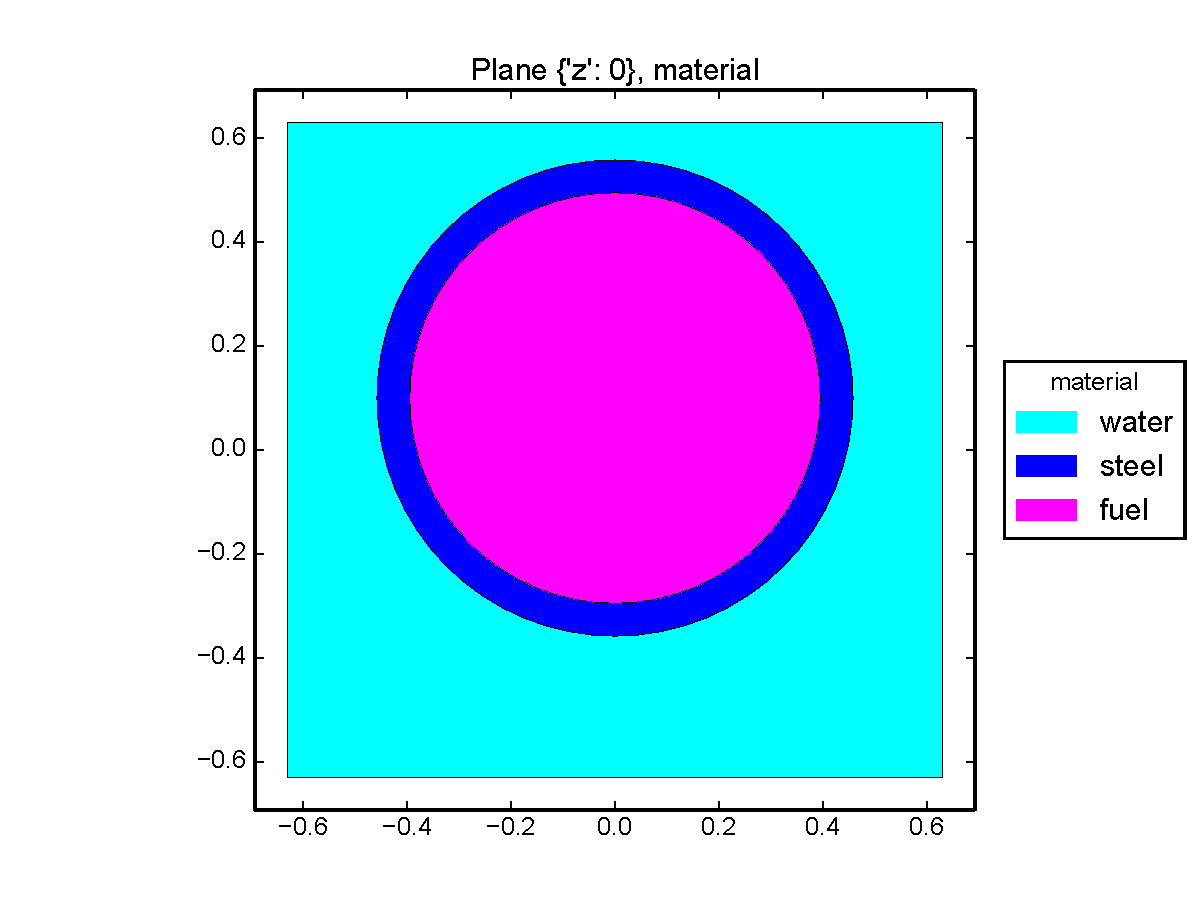
\includegraphics[width=\textwidth]{examples/ex2z.pdf}
        \column{0.5\textwidth}
            {\tiny x plane}
            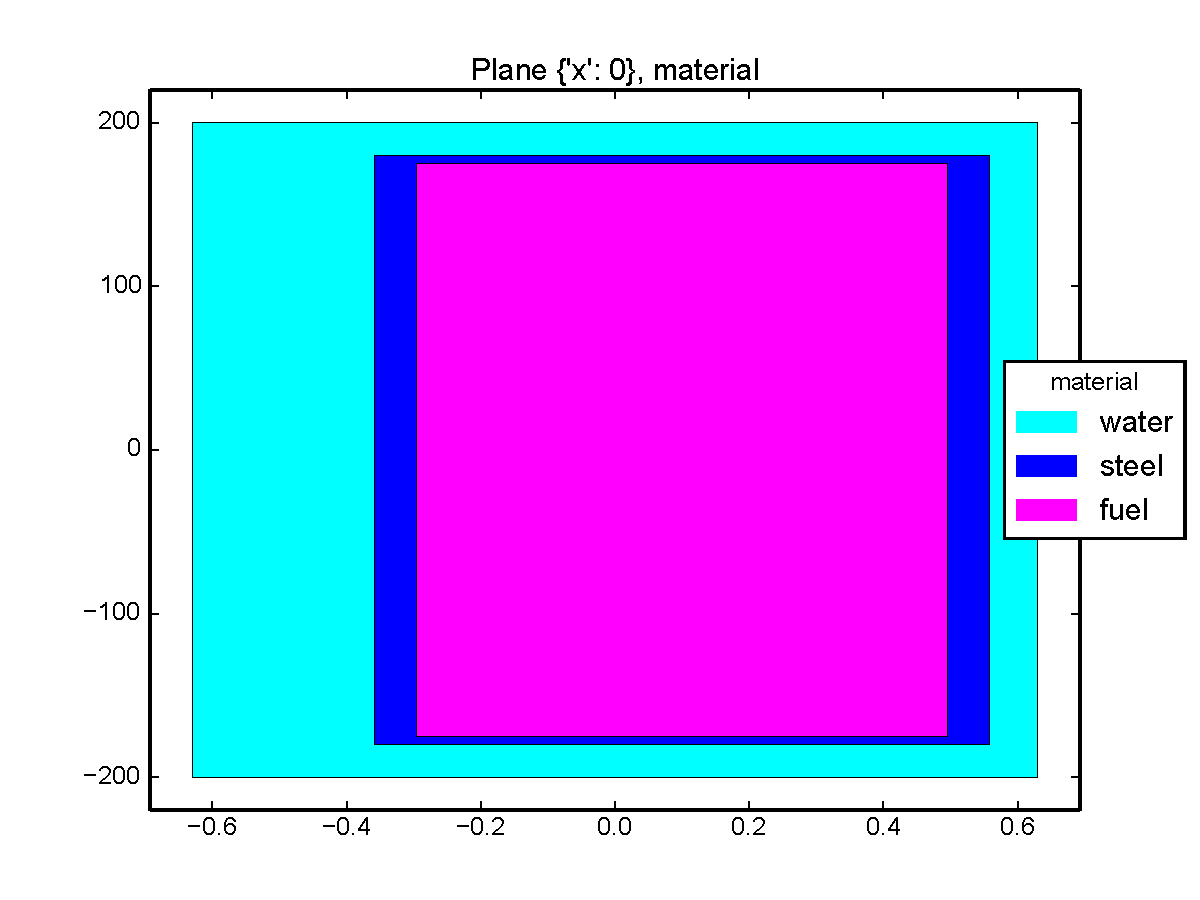
\includegraphics[width=\textwidth]{examples/ex2x.pdf}
    \end{columns}
\end{frame}

\subsection{Axial distributions}
\begin{frame}[fragile]
    \frametitle{Axial distributions}

    \begin{columns}
        \column{0.6\textwidth}
        \inputminted[frame=single,fontfamily=tt,fontsize=\tiny]{python}{examples/ex2_vars.py}

        \column{0.4\textwidth}{\scriptsize
        \begin{itemize}
            \item \pythoninline/get_child()/ method refers to one of the solids used in geometry definition. 
            \item each solid has \pythoninline/temp/, \pythoninline/dens/ and \pythoninline/heat/ attributes
                  to represent axial profiles of temperature, density and heat, respectively.
            \item \pythoninline/set_grid()/ method sets amount and relative thickness of axial mesh layers; first list element corresponds lower layer.

            \item \pythoninline/colormap()/ can generate colormaps of axial profiles.
        \end{itemize}
        }
     \end{columns}
\end{frame}

\begin{frame}[fragile]
    \frametitle{Plots}
    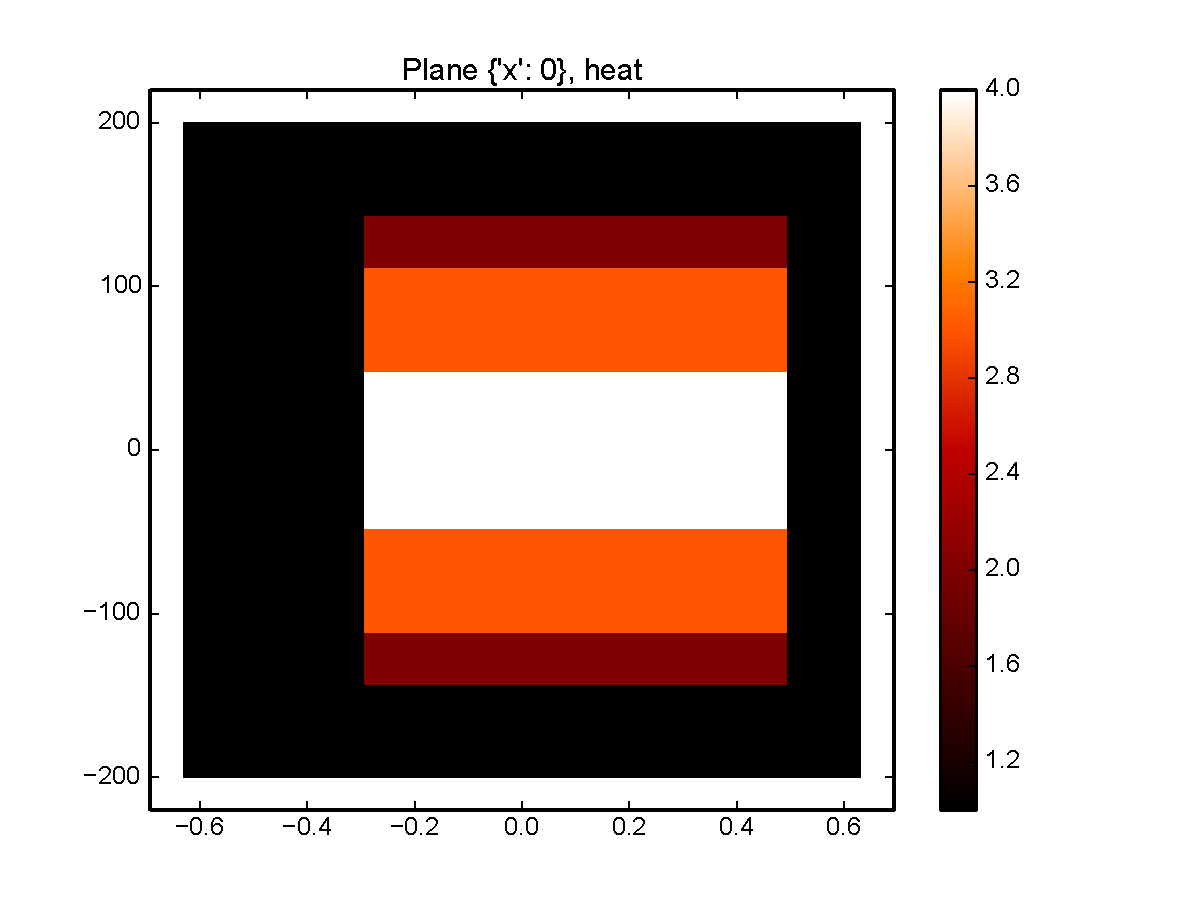
\includegraphics[width=0.5\textwidth]{examples/ex2t.pdf}
\end{frame}

\subsection{Coupled calculations}
\begin{frame}[fragile]
    \frametitle{Coupled calculations}

    \begin{columns}
        \column{0.6\textwidth}
        \inputminted[frame=single,fontfamily=tt,fontsize=\tiny]{python}{examples/ne4_coupl.py}

        \column{0.4\textwidth}{\scriptsize
        \begin{itemize}
            \item given geometry \pythoninline/a/ and code-specific data in \pythoninline/MI/ and \pythoninline/SI/ were already defined
            \item \pythoninline/run()/ method generates input, starts code, waits until it completes, reads results and returns copy of \pythoninline/a/ that contain in \pythoninline/heat/ attributes MCNP results.
        \end{itemize}
        }
     \end{columns}
\end{frame}


\subsection{Square lattices}
\begin{frame}[fragile]
    \frametitle{Square lattices}

    \begin{columns}
        \column{0.6\textwidth}
        \inputminted[frame=single,fontfamily=tt,fontsize=\tiny]{python}{examples/ex3_lat.py}

        \column{0.4\textwidth}{\scriptsize
        \begin{itemize}
            \item \pythoninline/grid/ attribute describes superimposed rectangular lattice, which can be used to
                position inserted solids.
            \item \pythoninline/grid.insert()/ method is similar to \pythoninline/insert()/ method, but inserted solid
                is placed in lattice element specified as 1-st agrument.
            \item \pythoninline/copy_tree()/ method returns deep copy of a solid (i.e. all inserted solids are copied as well)
            \item \pythoninline/grid.center()/ method positions lattice with respect to solid in a way that rectangle circumscribing all
                solids inserted into lattice elements, is centered.
        \end{itemize}
        }
     \end{columns}
\end{frame}

\begin{frame}[fragile]
    \frametitle{Plots}
    \begin{columns}
        \column{0.5\textwidth}
        {\tiny Lattice not centered: (0,0,0)-th element is at origin}
            \includegraphics[width=\textwidth]{examples/ex3_1.pdf}
        \column{0.5\textwidth}
        {\tiny After \pythoninline/grid.center()/ method}
            \includegraphics[width=\textwidth]{examples/ex3_2.pdf}
    \end{columns}
\end{frame}
% 
% 
% 
% 
\begin{frame}[fragile]
    \frametitle{Features of  high-level interfaces}
    \begin{itemize}
        \item Complex geometries can be defined with operations of insertion and translation with respect to container.

        \item MCNP high-level interface can handle any geometry (theoretically).
            \begin{itemize}
                \item \pythoninline/grid/ is modelled with lattices in MCNP input file
                \item solids are compared: equal solids represented using the same universe
                \item If possible, macrobodies are used
                \item non-trivial heat axial distributions considered as definition of heat deposition meshtally
                \item temperature axial meshes define \bashinline/tmp/ cell options and are used to find xs data. 
            \end{itemize}

        \item SCF high-level interface  is limited: 
            \begin{itemize}
                \item only square bundles of heated rods or unheated cylinder channels
                \item all solids in model must have same height
                \item coolant-centerd sub-channels are modelled in SCF, but
                \item rod-centered temperatures and densities are returned back to model
            \end{itemize}
    \end{itemize}
\end{frame}

\subsection{Material nuclide composition}
\begin{frame}[fragile]
    \frametitle{Compound materials}
    \begin{columns}
        \column{0.45\textwidth}
        \inputminted[frame=single,fontfamily=tt,fontsize=\scriptsize]{python}{examples/ex2_mat.py}
        \column{0.55\textwidth}{\scriptsize
        \begin{itemize}
            \item Materials can be multiplied by scalar and added 
            \item \pythoninline/thermal/ attribute specifies part of thermal data name. Particular table is chosen to fit temperature.
            \item \pythoninline/sdict/ dictionary specifies substitutions if cross-sections not available. 
            \item \pythoninline/card/ method returns multi-line string containg definition of material for MCNP input file. Can be used separately.
            \item Generally, \pythoninline/Material/ class constructor takes a list of tuples of the form \pythoninline/(spec, amount, unit)/, where
                \pythoninline/spec/ -- string, integer or Material instance, \pythoninline/amount/ -- amount of ingredient and \pythoninline/unit/ --flag specifying units.
        \end{itemize}
        }
     \end{columns}
\end{frame}
\begin{frame}[fragile]
    \frametitle{Compound materials, output}
    \begin{columns}
        \column{0.7\textwidth}
        \inputminted[frame=single,fontfamily=tt,fontsize=\tiny]{bash}{examples/ex2_mat.out}
        \column{0.3\textwidth}{\tiny
        \begin{itemize}
            \item Material \pythoninline/w/ contains nuclide O-18, but in MCNP material card it is substituted with O-16.
            \item Material card is formatting string, thus actual material numbers is simple to insert.
            \item Thremal data are chosen among cross-sections containing 'lwtr' in its name with closest temperature.
        \end{itemize}
        }
     \end{columns}
\end{frame}


\begin{frame}[fragile]
    \frametitle{Implicit material definition}
    {\scriptsize 
    Problem: Given U and Pu isotopic vectors in \% by weight, define MOX having
    10\% at. of fissile nuclides.
    }
    \begin{columns}
        \column{0.6\textwidth}
        \inputminted[frame=single,fontfamily=tt,fontsize=\tiny]{python}{examples/ex_mox.py}
        \column{0.4\textwidth}{\scriptsize
        \begin{itemize}
            \item U and Pu elements, \pythoninline/u/ and \pythoninline/p/, are defined using grams.
            \item Initially, \pythoninline/mox/ is defined using equal amounts (moles) of U and Pu oxide.
            \item Objective function \pythoninline/of()/ takes a material instance as argument and returns deviation of ratio of 
                fissile nuclides to all heavy metal nucled from 5\% 
            \item Method \pythoninline/tune()/ changes amount of specified ingredients until objective function returns (almost) zero.
        \end{itemize}
        }
     \end{columns}
\end{frame}
\begin{frame}[fragile]
    \frametitle{Implicit material definition, output}
    \begin{columns}
        \column{0.7\textwidth}
        \inputminted[frame=single,fontfamily=tt,fontsize=\tiny]{bash}{examples/ex_mox.out}
        \column{0.3\textwidth}{\scriptsize
        After \pythoninline/tune()/ method, amount of fissile nuclides is 0.0347 mol and amount of all heavy metal nuclides is 0.347 mol in
        definition of \pythoninline/mox/ material.
        }
     \end{columns}
\end{frame}
